\documentclass[crop,class=article]{standalone}
%----------------------------Preamble-------------------------------%
\usepackage{pgfplots, tikz}             % Drawing/graphing tools.
\pgfplotsset{compat=1.9}                % Version of pgfplots.
%--------------------------Main Document----------------------------%
\begin{document}
    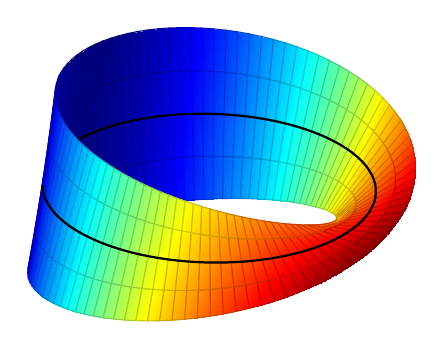
\begin{tikzpicture}
        \begin{axis}[
            hide axis,
            view={40}{40}
        ]
            \addplot3[%
                surf,
                shader=faceted interp,
                point meta=x,
                colormap/jet,
                samples=100,
                samples y=5,
                domain=0:360,
                y domain=-0.5:0.5
            ]   ({(1+0.5*y*cos(x/2)))*cos(x)},
                 {(1+0.5*y*cos(x/2)))*sin(x)},
                 {0.5*y*sin(x/2)});

            \addplot3[%
                samples=100,
                domain=-140:180,
                samples y=0,
                thick,
                line cap=round
            ]   ({cos(x)},{sin(x)},{0});
        \end{axis}
    \end{tikzpicture}
\end{document}